\section{Celdas Universales}

En esta secci\'on se analizan distintas celdas universales, es decir, celdas de configuraciones diferentes que est\'an compuestas por dos integradores. Las celdas en estudio son la Kerwin-Huelsman-Newcomb, la Tow-Thomas, la Ackerberg-Mossberg y la Fleischer-Tow. La finalidad de dicho an\'alisis es luego realizar un filtro rechaza banda a partir de una aproximaci\'on de Chebychev Inverso que cumpla las siguientes especificaciones:

	\begin{table}[H]
	\centering
	\begin{tabular}{c c}
		\hline
		$f_\infty$ & $51kHz$ \\ 
		notch depth &  $\geq 50dB$\\
		$\Delta f_a$ & $600Hz$\\
		$\Delta f_p$ & $10kHz$\\
		$A_a$ & $40dB$\\
		$A_p$ & $6dB$\\
		$G$ & $[-3:3]dB$\\
		$|Zin(f)|$ & $\geq 50k\Omega$\\	
		Cantidad de ceros de transmisi\'on & $\geq 2$\\
		\hline
	\end{tabular}
	\caption{Especificaciones del filtro rechaza banda a realizar.}
	\label{especificaciones}
\end{table}

El an\'alisis que se llevar\'a a cabo para cada celda es tanto ideal como real, para poder comprender las caracter\'isticas que determinar\'an si es posible o no implementar cada celda para lograr el filtro especificado. Una vez determinadas las ventajas y desventajas de cada celda frente al filtro que se desea realizar, se har\'a un mayor enfoque en la celda elegida para llevar el filtro a la pr\'actica.


\todo{ver si esto queda o no}
\subsection{Introducci\'on te\'orica}

Se comienza analizando el comportamiento de circuitos compuestos por dos integradores, representandolos mediante diagramas en bloques. El siguiente diagrama de la figura \ref{int1}\footnote{Adaptaci\'on de una imagen obtenida de: https://elxcompacme.files.wordpress.com/2014/03/filter-kendell-su.pdf} es una representaci\'on simple que permite entender lo que se desarrolla luego.

\begin{figure}[H] %!ht
	\centering
	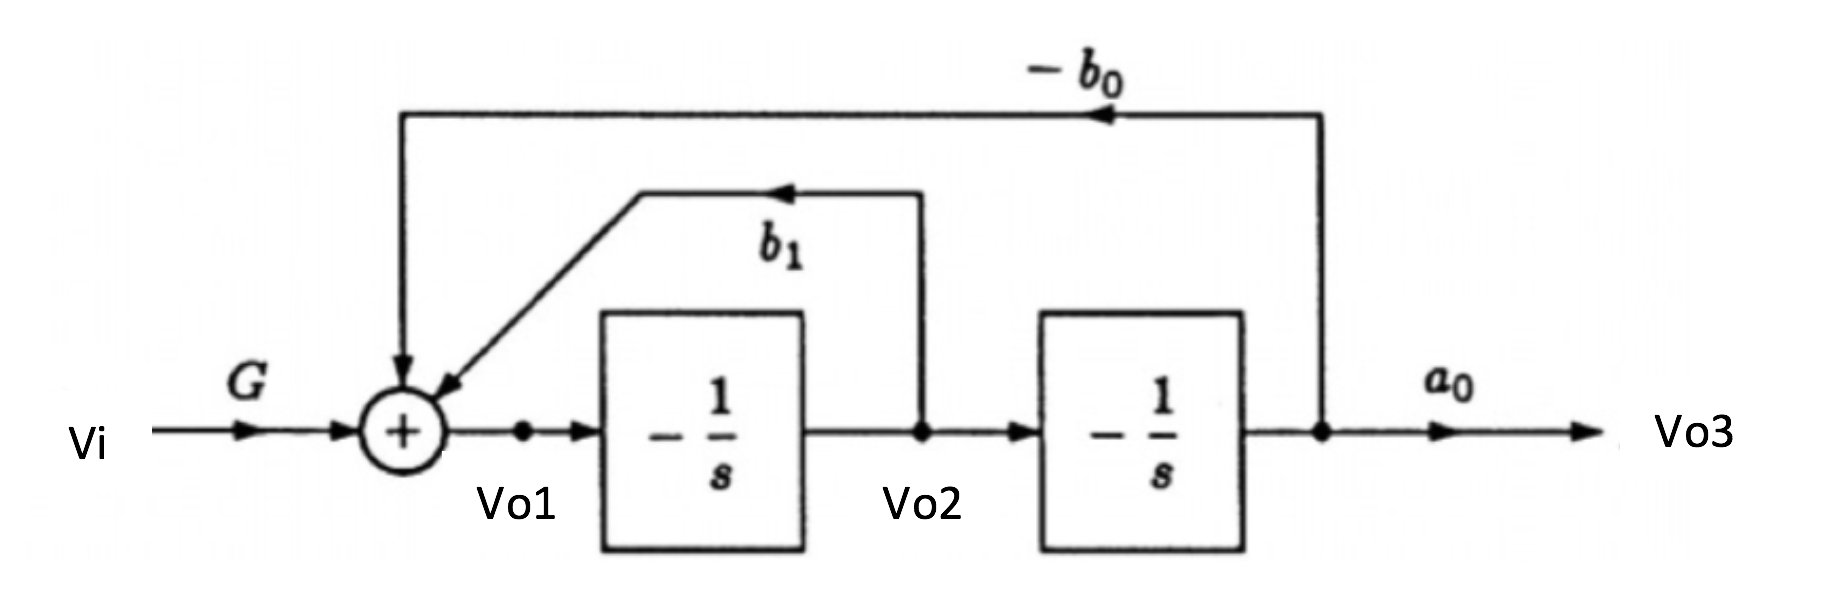
\includegraphics[width=12cm,height=12cm,keepaspectratio]{../EJ4/imagenes/int1.png}
	\caption{Representaci\'on en bloques de un circuito simple de segundo orden formado por dos integradores.}
	\label{int1}
\end{figure}

Del diagrama anterior, se obtienen las siguientes expresiones, a partir de las cuales se puede apreciar que se trata de un circuito de orden 2.

\begin{equation}
\begin{cases}
	Vo_2 = -\frac{1}{2} \cdot Vo_1\\
	Vo_3 = -\frac{1}{2} \cdot Vo_2\\
	H(s) = \frac{Vo_3}{V_i} = G \cdot \frac{a_0}{s^2 + b_1 s + b_0}
	\label{int2eq}
\end{cases}
\end{equation}

Si ahora se suman a la salida las tensiones $Vo_1$ y $Vo_2$ como se muestra en el diagrama de la siguiente figura \ref{int2}:

\begin{figure}[H] %!ht
	\centering
	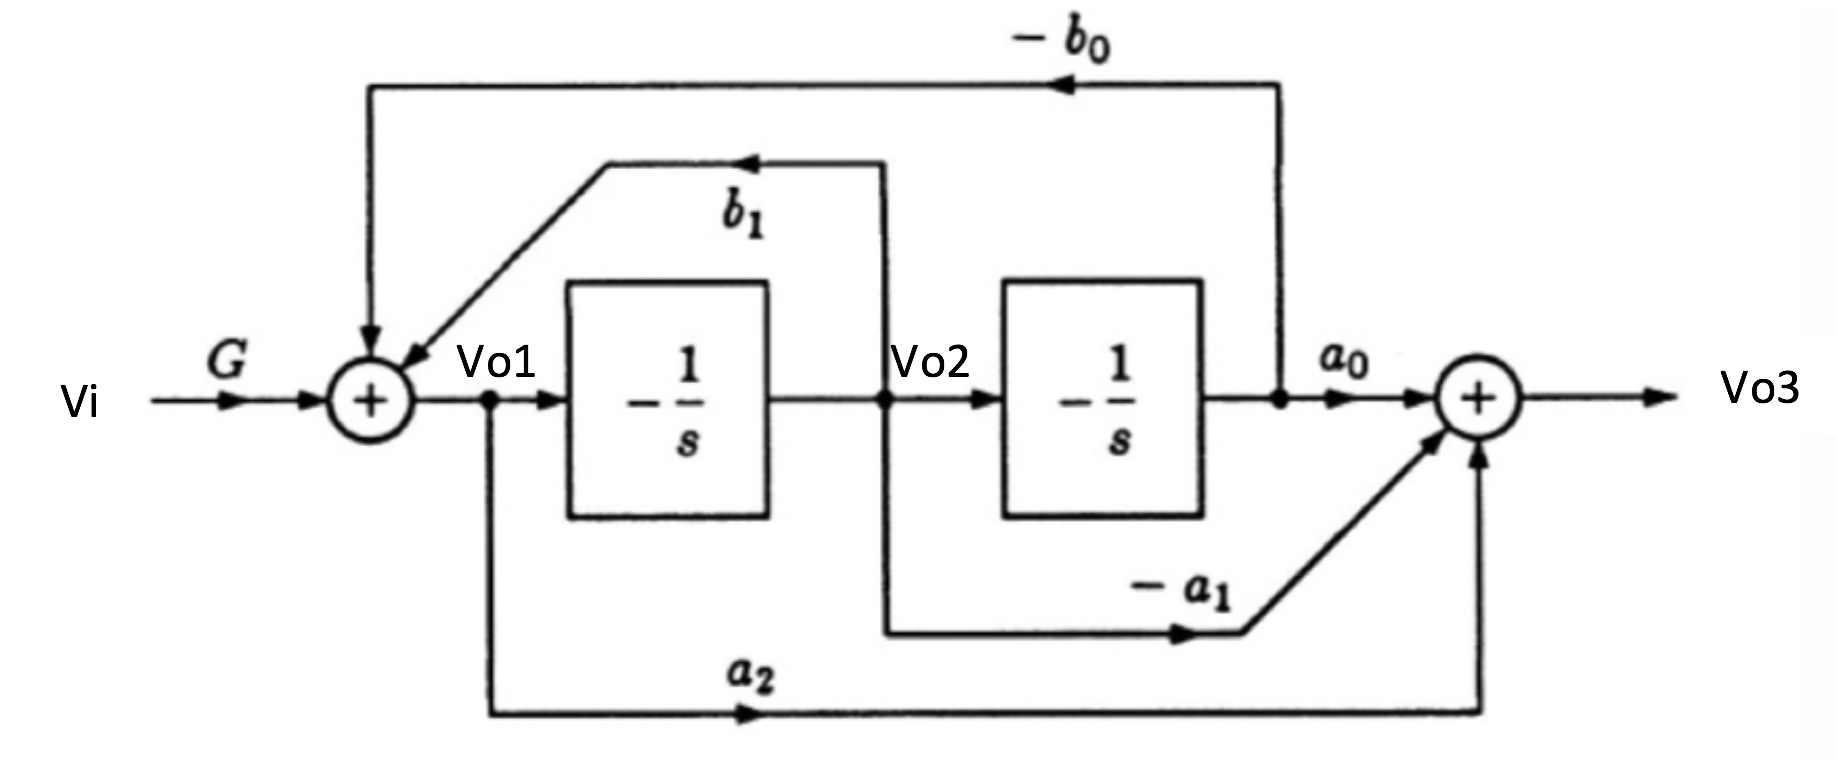
\includegraphics[width=12cm,height=12cm,keepaspectratio]{../EJ4/imagenes/int2.png}
	\caption{Misma representaci\'on en bloques que antes pero sumando las tensiones $Vo_1$ y $Vo_2$ a la salida.}
	\label{int2}
\end{figure}

As\'i se obtiene:

\begin{equation}
	\frac{Vo_3}{Vi} = G \cdot \frac{a_2s^2+a_1s+a_0}{s^2+b_1s+b_0}
	\label{int2eq}
\end{equation}

Las configuraciones que se analizan a continuaci\'on est\'an basadas en modificaciones sobre este \'ultimo diagrama de la figura \ref{int2} y su ecuaci\'on correspondiente \ref{int2eq}

\subsection{Configuraciones correspondientes a distintas celdas universales: An\'alisis ideal}

A continuaci\'on se detallan las configuraciones de las cuatro celdas universales previamente enunciadas. Junto a la configuraci\'on circuital de cada una de estas celdas, se presenta su funci\'on transferencia, la ganancia $G$, los par\'ametros $Q$ y $\omega_0$; y sus sensibilidades relativas respecto a cada componente que conforma el circuito. Para esto, se hace un an\'alisis en el que los amplificadores operacionales son considerados ideales. Es decir, se considera que cada amplificador operacional cuenta con las siguientes caracter\'isticas:

\begin{equation}
	\begin{cases}
		Z_{in} \to \infty\\
		A_{VOL} \to \infty\\
		Z_{out} \to 0\Omega\\
		I_{in+} = I_{in-} = 0A
		
	\end{cases}
\end{equation}


\todo{citar la pagina esta de internet}
\footnote{https://elxcompacme.files.wordpress.com/2014/03/filter-kendell-su.pdf}
\subsection{Celda 2do orden Kerwin-Huelsman-Newcomb (KHN): An\'alisis ideal}


\begin{figure}[H] %!ht
	\centering
	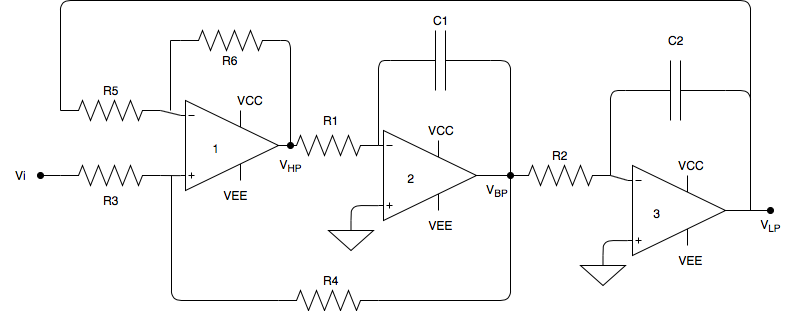
\includegraphics[width=12cm,height=12cm,keepaspectratio]{../EJ4/imagenes/KERWIN.png}
	\caption{Circuito Kerwin-Huelsman-Newcomb}
	\label{kerwin}
\end{figure}

\subsubsection{Funci\'on transferencia y par\'ametros}
\begin{table}[h!]
	\centering
	\begin{tabular}{c c c c c}
		Salida & $H(s)$ & $G$ & $\omega_0$ & $Q$\\
		\hline \\
		LP & $\frac{\frac{R_4}{R_5R_1R_2C_1C_2}\cdot \frac{R_5+R_6}{R_3+R_4}}{S^2+\frac{R_3}{R_5R_1C_1}\cdot \frac{R_5+R_6}{R_3+R_4}s+\frac{R_6}{R_5R_1R_2C_1C_2}}$& $\frac{R_4 (R_5+R_6)}{R_6(R_3+R_4)}$& \multirow{7}{*}{$\sqrt{\frac{R_4 (R_5+R_6)}{R_6(R_3+R_4)}}$}&
		\multirow{7}{*}{$\frac{R_5(R_3+R_4)}{R_3(R_5+R_6)}\cdot \sqrt{\frac{R_6R_1C_1}{R_5R_2C_2}}$}\\ \\
		BP & $- \frac{\frac{R_4}{R_5R_1C_1}\cdot \frac{R_5+R_6}{R_3+R_4} s}{S^2+\frac{R_3}{R_5R_1C_1}\cdot \frac{R_5+R_6}{R_3+R_4}s+\frac{R_6}{R_5R_1R_2C_1C_2}}$&$-\frac{R_4}{R_3}$& &\\ \\
		HP& $- \frac{\frac{R_4}{R_5}\cdot \frac{R_5+R_6}{R_3+R_4} S^2}{S^2+\frac{R_3}{R_5R_1C_1}\cdot \frac{R_5+R_6}{R_3+R_4}s+\frac{R_6}{R_5R_1R_2C_1C_2}}$& $\frac{R_4(R_5+R_6)}{R_5(R_3+R_4)}$& & \\ \\
		\hline
	\end{tabular}
	\caption{Caracter\'isticas de la celda Kerwin-Huelsman-Newcomb.}
	\label{hg_tt}
\end{table}

\subsubsection{Sensibilidades}

\begin{table}[H]
	\centering
	\begin{tabular}{c c c c c c}
		  & $\omega_0$ & $Q$ &$G_{LP}$ & $G_{BP}$& $G_{HP}$\\
		\hline \\
	$R_1$ & $-\frac{1}{2}$& $\frac{1}{2}$ & $0$& $0$&$0$\\ \\
	$R_2$ & $-\frac{1}{2}$& $-\frac{1}{2}$ & $0$& $0$& $0$\\ \\
	$R_3$ & $0$& $-\frac{R_4}{R_3+R_4}$ & $-\frac{R_3}{R_3+R_4}$&$-1$ & $-\frac{R_3}{R_3+R_4}$\\ \\
	$R_4$ & $0$& $\frac{R_4}{R_3+R_4}$& $\frac{R_3}{R_3+R_4}$ &$1$ & $\frac{R_3}{R_3+R_4}$\\ \\
	$R_5$ & $-\frac{1}{2}$&$\frac{R_6-R_5}{2(R_5+R_6)}$ & $\frac{R_5}{R_5+R_6}$&$0$ & $-\frac{R_6}{R_5+R_6}$\\ \\
	$R_6$ & $\frac{1}{2}$& $-\frac{R_6-R_5}{2(R_5+R_6)}$ & $-\frac{R_5}{R_5+R_6}$& $0$&$\frac{R_6}{R_5+R_6}$ \\ \\
	$C_1$ & $-\frac{1}{2}$& $\frac{1}{2}$ & $0$& $0$&$0$ \\ \\
	$C_2$ & $-\frac{1}{2}$& $-\frac{1}{2}$ & $0$ & $0$&$0$\\ \\
		\hline
	\end{tabular}
	\caption{Sensibilidades de la celda Kerwin-Huelsman-Newcomb.}
	\label{sens_k}
\end{table}


Esta celda tiene sensibilidades bajas.

\subsubsection{Impedancia de entrada}
\todo{completar}


\subsubsection{Impedancia de salida}
La salida del circuito se encuentra a la salida de un amplificador operacional con realimentaci\'on negativa.  Se indic\'o previamente que la impedancia de salida de un amplificador operacional ideal es $Z_{out} \to 0$, lo que implica que la impedancia de salida del circuito tambi\'en tienda a cero.

\begin{equation}
\begin{cases}
Vo_2 = -\frac{1}{2} \cdot Vo_1\\
Vo_3 = -\frac{1}{2} \cdot Vo_2\\
H(s) = \frac{Vo_3}{V_i} = G \cdot \frac{a_0}{s^2 + b_1 s + b_0}
\label{int2eq}
\end{cases}
\end{equation}

\todo{CHEQUEAR circuito porque en el palombo est\'a distinto!}

Dependiendo de d\'onde se tome la salida del circuito \ref{kerwin}, se puede obtener un filtro pasa altos, un pasa banda o un pasabajos. Lo que sucede con Kerwin-Huelsman-Newcomb es que no brinda una salida rechaza banda. La misma puede igual lograrse agregandole al circuito \ref{kerwin} un sumador, como se muestra en la figura \ref{sumador_extra}:

\begin{figure}[H] %!ht
	\centering
	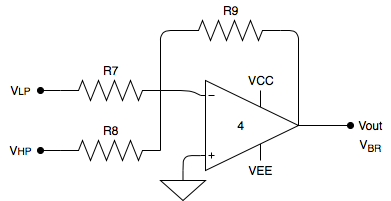
\includegraphics[width=8cm,height=8cm,keepaspectratio]{../EJ4/imagenes/sumador_extra.png}
	\caption{Sumador que se le agrega a la selda para obtener un rechaza banda.}
	\label{sumador_extra}
\end{figure}

\subsection{Celda 2do orden Tow-Thomas:An\'alisis ideal}

La celda Tow-Thomas var\'ia frente a la Kerwin-Huelsman-Newcomb al tener juntos a la entrada el sumador y el primer integrador, agregando luego un inversor y una resistencia en la realimentación que va de la salida $V_{LP}$ a la entrada del circuito. Esta nueva configuraci\'on, al igual que en la Kerwin-Huelsman-Newcomb sigue teniendo una salida de pasa bajos y una de pasa banda, pero ya no tiene una de pasa altos. 

\begin{figure}[H] %!ht
	\centering
	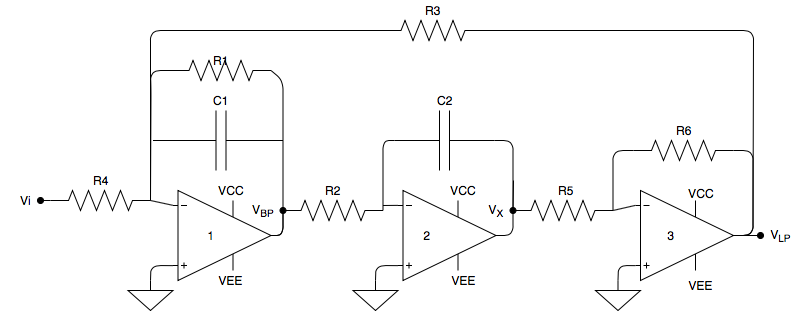
\includegraphics[width=12cm,height=12cm,keepaspectratio]{../EJ4/imagenes/TOW-THOMAS.png}
	\caption{Celda Tow-Thomas}
	\label{tow_thomas}
\end{figure}

\subsubsection{Funci\'on transferencia y par\'ametros}
Los par\'ametros correspondientes a la celda Tow-Thomas son los siguientes:

\begin{table}[H]
	\centering
	\begin{tabular}{c c c c c}
		Salida & $H(s)$ & $G$ & $\omega_0$ & $Q$\\
		\hline \\
		LP & $-\frac{\frac{R_6/R_5}{R_2R_4C_1C_2}}{s^2+\frac{1}{R_1C_1}+\frac{R_6/R_5}{R_2R_3C_1C_2}}$& $- \frac{R_3}{R_4}$& \multirow{4}{*}{$\sqrt{\frac{R_6/R_5}{R_2R_3C_1C_2}}$}&
		\multirow{4}{*}{$\frac{R_1}{\sqrt{R_2R_3}}\sqrt{\frac{R_6C_1}{R_5C_2}}$}\\ \\
		BP & $-\frac{\frac{1}{R_4 C_1}s}{s^2+\frac{1}{R_1C_1}+\frac{R_6/R_5}{R_2R_3C_1C_2}}$&$-\frac{R_1}{R_4}$& &\\ \\
		\hline
	\end{tabular}
	\caption{Caracter\'isticas de la celda Tow-Thomas.}
	\label{hg_tt}
\end{table}

\subsubsection{Sensibilidades}
\begin{table}[H]
	\centering
	\begin{tabular}{c c c c c }
		& $\omega_0$ & $Q$ &$G_{LP}$ & $G_{BP}$\\
		\hline \\
		$R_1$ & $0$& $1$ & $0$& $1$\\ \\
		$R_2$ & $-\frac{1}{2}$& $-\frac{1}{2}$ & $0$& $0$\\ \\
		$R_3$ & $-\frac{1}{2}$& $-\frac{1}{2}$ & $1$&$0$ \\ \\
		$R_4$ & $0$& $0$& $-1$ &$-1$ \\ \\
		$R_5$ & $-\frac{1}{2}$&$-\frac{1}{2}$ & $0$&$0$ \\ \\
		$R_6$ & $\frac{1}{2}$& $\frac{1}{2}$ & $0$& $0$ \\ \\
		$C_1$ & $-\frac{1}{2}$& $\frac{1}{2}$ & $0$& $0$\\ \\
		$C_2$ & $-\frac{1}{2}$& $-\frac{1}{2}$ & $0$ & $0$\\ \\
		\hline
	\end{tabular}
	\caption{Sensibilidades de la celda Tow-Thomas.}
	\label{sens_tt}
\end{table}

\subsubsection{Impedancia de entrada}
\todo{COMPLETAR}

\subsubsection{Impedancia de salida}
Al igual que para la celda anterior, como la impedancia de salida del circuito es tomada a la salida de un amplificador operacional y dado que este es considerado ideal, la impedancia de salida del circuito tiende a cero.

\subsection{Celda 2do orden Ackerberg-Mossberg: An\'alisis ideal}

\begin{figure}[H] %!ht
	\centering
	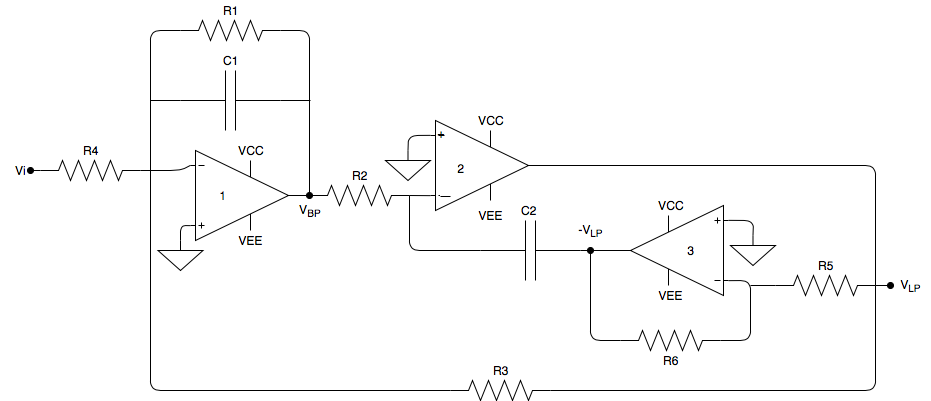
\includegraphics[width=12cm,height=12cm,keepaspectratio]{../EJ4/imagenes/ACKBERG.png}
	\caption{Celda Ackerberg-Mossberg}
	\label{ackerberg}
\end{figure}

\subsubsection{Funci\'on transferencia y par\'ametros}

\begin{table}[H] %estas son las del libro!
	\centering
	\begin{tabular}{c c c c c}
		Salida & $H(s)$ & $G$ & $\omega_0$ & $Q$\\
		\hline \\
		LP & $- \frac{\frac{R_5}{C_1C_2R_2R_4R_6}}{s^2+\frac{1}{C_1R_1}s+\frac{R_5}{C_1C_2R_2R_3R_6}}$& $-\frac{R_3}{R_4}$& \multirow{4}{*}{$\sqrt{\frac{R_5}{C_1C_2R_2R_3R_6}}$}&
		\multirow{4}{*}{$C_1R_1\sqrt{\frac{R_5}{C_1C_2R_2R_3R_6}}$}\\ \\
		BP & $-\frac{\frac{1}{C_1R_4}s}{s^2+\frac{1}{C_1R_1}s + \frac{R_5}{C_1C_2R_2R_3R_6}}$&$-\frac{R_1}{R_4}$& &\\ \\
		\hline
	\end{tabular}
	\caption{Caracter\'isticas de la celda Ackerberg-Mossberg.}
	\label{am_tt}
\end{table}

\subsubsection{Sensibilidades}

\todo{chequear sensibilidad Q respecto a c1}
\begin{table}[H]
	\centering
	\begin{tabular}{c c c c c }
		& $\omega_0$ & $Q$ &$G_{LP}$ & $G_{BP}$\\
		\hline \\
		$R_1$ & $0$ & $1$ & $0$ & $1$\\ \\
		$R_2$ & $-\frac{1}{2}$ & $-\frac{1}{2}$ & $0$ & $0$\\ \\
		$R_3$ & $-\frac{1}{2}$ & $-\frac{1}{2}$ & $1$ & $0$ \\ \\
		$R_4$ & $0$ & $0$ & $-1$ & $-1$ \\ \\
		$R_5$ & $\frac{1}{2}$ & $\frac{1}{2}$ & $0$ & $0$ \\ \\
		$R_6$ & $-\frac{1}{2}$ & $-\frac{1}{2}$ & $0$ & $0$ \\ \\
		$C_1$ & $-\frac{1}{2} $ & $\frac{1}{2}$ & $0$ & $0$\\ \\
		$C_2$ & $-\frac{1}{2}$ & $-\frac{1}{2}$ & $0$ & $0$\\ \\
		\hline
	\end{tabular}
	\caption{Sensibilidades de la celda Ackerberg-Mossberg.}
	\label{sens_am}
\end{table}

\subsubsection{Impedancia de entrada}
\todo{completar}

\subsubsection{Impedancia de salida}
Esta celda tambi\'en presenta una impedancia de salida igual a cero al considerar los amplificadores operacionales como ideales, debido a que la salida del circuito es tomada a la salida de un amplificador operacional.

\subsubsection{Celda 2do orden Fleischer-Tow: An\'alisis ideal}

Una caracter\'istica importante a remarcar de la selda Flesicher-Tow es que, a diferencia de las celdas anteriores, permite realizar cualquier tipo de filtro de segundo orden sin la necesidad de agregar otro amplificador operacional. Como se ha estudiado en trabajos pr\'acticos anteriores, el amplificador operacional tiene ciertas limitaciones para un circuito, debidas al slew rate, a la saturaci\'on, entre otras; por lo que es ventajoso el hecho de no tener que agregar un amplificador operacional para obtener un filtro rechaza banda.


\begin{figure}[H] %!ht
	\centering
	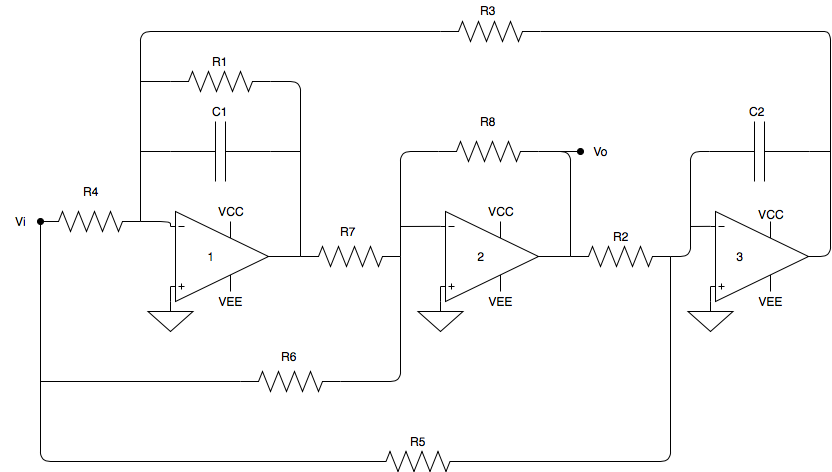
\includegraphics[width=12cm,height=12cm,keepaspectratio]{../EJ4/imagenes/FLEISCHER.png}
	\caption{Celda Fleischer-Tow}
	\label{fleischer}
\end{figure}

\subsubsection{Funci\'on transferencia y par\'ametros}

\begin{table}[H] %estas son las del libro!
	\centering
	\begin{tabular}{c c c c}
		$H(s)$ gen\'erica & $\omega_0$ & $Q$\\
		\hline \\
		 $- \frac{\frac{R_8}{R_6}s^2+\left(\frac{R_8}{R_6R_1C_1}-\frac{R_8}{R_4R_7C_1}\right)s+\frac{R_8}{R_3R_5R_7C_1C_2}}{s^2+\frac{1}{R_1C_1}s+\frac{R_8}{R_2R_3R_7C_1C_2}}$&$\sqrt{\frac{R_8}{R_2R_3R_7C_1C_2}}$&$R_1C_1\sqrt{\frac{R_8}{R_2R_3R_7C_1C_2}}$\\ \\
		\hline
	\end{tabular}
	\caption{Expresiones gen\'ericas de la celda Fleischer-Tow.}
	\label{f_generica}
\end{table}

\begin{table}[H] %estas son las del libro!
	\centering
	\begin{tabular}{c c c c c c}
		Salida & Condiciones & $H(s)$ & $G$ & $\omega_0$ & $Q$\\
		\hline \\
		LP&$R_6=R_4=\infty$ &$- \frac{\frac{R_8}{R_3R_5R_7C_1C_2}}{s^2+\frac{1}{R_1C_1}s+\frac{R_8}{R_2R_3R_7C_1C_2}}$& $-\frac{R_2}{R_5}$& \multirow{9}{*}{$\sqrt{\frac{R_8}{R_2R_3R_7C_1C_2}}$}&
		\multirow{9}{*}{$R_1C_1\sqrt{\frac{R_8}{R_2R_3R_7C_1C_2}}$}\\ \\
		BP &$R_6=R_5=\infty$  &$ \frac{\left(\frac{R_8}{R_4R_7C_1}\right)s}{s^2+\frac{1}{R_1C_1}s+\frac{R_8}{R_2R_3R_7C_1C_2}}$&$\frac{R_1R_8}{R_4R_7}$& &\\ \\
		HP & $R_5=\infty$&\multirow{2}{*}{$- \frac{\frac{R_8}{R_6}s^2}{s^2+\frac{1}{R_1C_1}s+\frac{R_8}{R_2R_3R_7C_1C_2}}$}&\multirow{2}{*}{$-\frac{R_8}{R_6}$}& &\\ 
		&$R_1R_6=R_4R_7$ & & & &\\ \\
		BR &$R_1R_6=R_4R_7$ &\multirow{2}{*}{$- \frac{\frac{R_8}{R_6}s^2+\frac{R_8}{R_3R_5R_7C_1C_2}}{s^2+\frac{1}{R_1C_1}s+\frac{R_8}{R_2R_3R_7C_1C_2}}$}&\multirow{2}{*}{$-\frac{R_2}{R_5}$}& &\\ \\ \\
		\hline
	\end{tabular}
	\caption{Caracter\'isticas de la celda Fleischer-Tow.}
	\label{f_cars}
\end{table}

\subsubsection{Sensibilidades}

\todo{ver si agregar los tipos de notch}
\begin{table}[H]
	\centering
	\begin{tabular}{c c c c c c c}
		& $\omega_0$ & $Q$ &$G_{LP}$ & $G_{BP}$& $G_{HP}$& $G_{BR}$\\
		\hline \\ 
		$R_1$ & $0$ & $1$ & $0$ & $1$ & $0$ & $0$\\ \\
		$R_2$ & $-\frac{1}{2}$ & $-\frac{1}{2}$ & $1$ & $0$ & $0$ & $1$\\ \\
		$R_3$ & $-\frac{1}{2}$ & $-\frac{1}{2}$ & $0$ & $0$ & $0$ & $0$\\ \\
		$R_4$ & $0$ & $0$ & $0$ & $-1$ & $0$ & $0$\\ \\
		$R_5$ & $0$ & $0$ & $-1$ & $0$ & $0$ & $-1$\\ \\
		$R_6$ & $0$ & $0$ & $0$ & $0$ & $-1$ & $0$\\ \\
		$R_7$ & $-\frac{1}{2}$ & $-\frac{1}{2}$ & $0$ & $-1$ & $0$ & $0$\\ \\
		$R_8$ & $\frac{1}{2}$ & $\frac{1}{2}$ & $0$ & $1$ & $1$ & $0$\\ \\
		$C_1$ & $-\frac{1}{2}$ & $\frac{1}{2}$ & $0$ & $0$ & $0$ & $0$\\ \\
		$C_2$ & $-\frac{1}{2}$ & $-\frac{1}{2}$ & $0$ & $0$ & $0$ & $0$\\ \\
		\hline
	\end{tabular}
	\caption{Sensibilidades de la celda Fleischer-Tow}
	\label{sens_am}
\end{table}

\subsection{Dise\~no de filtro rechaza banda mediante la aproximaci\'on  Chebychev Inverso}

\subsubsection{Especificaciones del filtro y aproximaci\'on}
A continuaci\'on se transcribe la tabla que cuenta con las especificaciones del filtro a realizar, que fue introducida al inicio de esta secci\'on, para facilitar la lectura y la comprensi\'on del an\'alisis que sigue.

	\begin{table}[H]
	\centering
	\begin{tabular}{c c}
		\hline
		$f_\infty$ & $51kHz$ \\ 
		notch depth &  $\geq 50dB$\\
		$\Delta f_a$ & $600Hz$\\
		$\Delta f_p$ & $10kHz$\\
		$A_a$ & $40dB$\\
		$A_p$ & $6dB$\\
		$G$ & $[-3:3]dB$\\
		$|Zin(f)|$ & $\geq 50k\Omega$\\	
		Cantidad de ceros de transmisi\'on & $\geq 2$\\
		\hline
	\end{tabular}
	\caption{Especificaciones del filtro rechaza banda a realizar.}
	\label{especificaciones2}
\end{table}

La finalidad de implementar un filtro a partir de una aproximaci'on es adquirir presici\'on y selectividad, como lo son las especificaciones de la tabla \ref{especificaciones2}. Al aumentar la selectividad de un filtro, el mismo deja de poder ser realizado con un solo filtro de orden 1 \'o 2, y es as\'i como surge la necesidad de usar un filtro de un orden mayor. Para esto, existen distintas aproximaciones que permiten no solo realizar un filtro de orden mayor, si no que adem\'as brindan la posibildiad de realizar un filtro de orden mayor a dos a partir de la conexi\'on en cascada de varios filtros de orden 2 \'o 1, cuya cantidad depende del orden del circuito completo. Se pidi\'o que el filtro fuera obtenido con la aproximaci\'on de Chebychev IInverso (Chebychev II) y que el filtro tuviera por lo menos dos ceros de transmisi\'on. La arpoximaci\'on de Chevychev Inverso exige la presencia de ceros de transmisi\'on, es decir, ceros ubicados sobre el eje imaginario (el eje $j\omega$) de la frecuencia. 

\todo{PONER todo lo de cheby. formulas y resultados obtenidos, los q, orden, polos etc.}


\subsubsection{Selección de celda y dise\~no de etapas}
Previamente fueron mostradas las caracter\'isticas de cada celda. Para obtener un notch, es necesario emplear una celda que tenga una salida de notch, o bien utilizar una salida pasa bajos sumada con una pasa altos. Ya que la celda Tow-Thomas y la Ackerberg-Mossberg presentan únicamente salida pasabajos y pasabanda, no se empleará dicha celda al no tener la posibilidad de formar un notch, debido a que no tienen una salida pasa altos. Por lo tanto las opciones son la celda \todo{seguir}

\subsubsection{Celda 2do orden Fleischer-Tow: An\'alisis real}

\subsubsection{Simulaci\'on y verificaci\'on}

\subsubsection{Dise\~o de PCB}

\subsubsection{Resultados obtenidos}

\subsection{Conclusiones} 
